\documentclass[10pt,letterpaper]{article}

\usepackage[top=2cm,right=2cm,bottom=2cm,left=2cm,nohead,nofoot]{geometry}

\usepackage{amsmath}
\usepackage{graphicx}
\usepackage{indentfirst}
\usepackage{url}
\usepackage{mdwlist}
\usepackage[compact]{titlesec}
\usepackage[T1]{fontenc}
\usepackage{palatino}
\usepackage[brazil]{babel}
\usepackage[utf8]{inputenc}
\usepackage{enumerate}

\pagestyle{empty}
\setcounter{secnumdepth}{5}

\makeatletter
\def\thickhrulefill{\leavevmode \leaders \hrule height 1pt\hfill \kern \z@}
\renewcommand{\maketitle}{
	\begingroup
		\parindent \z@
		\begin{center}
			{\normalsize \@author\par}%
			\thickhrulefill\par
			{\small\raggedleft \@date\par}%
			{\Large\raggedright \@title\par}%
		\end{center}%
	\endgroup
}
\makeatother

\title{F 429: Experimento II}
\author{033910 Leandro Mendes | 104198 Thiago Verratti | 118451 Rafael Mendes | 121096 Leonardo Sorensen}
\begin{document}
\maketitle
\tableofcontents
\listoffigures
\listoftables
\newpage
\section{Introdução}
Este experimento propõe-se a estudar as experimentalmente e analizar as formas de onda dos circuitos integrador e
diferenciador. Neste caso, são do tipo RC e compostos por uma fonte, um resistor e um
capacitor ligados em série.\\
Analisamos também transientes em circuito ressonante série RLC. Os transientes podem ser estudados no laboratório excitando o circuito com uma onda quadrada de período muito maior que a constante de tempo do circuito.
\section{Metodologia}
\subsection{Instrumentos e Componentes}
Os instrumentos e componentes utilizados estão listados abaixo com seus respectivos valores nominais.
\begin{itemize}
\item{Gerador de Funções Tektronix CFG 253.} 
\item{Osciloscópio digital Tektronix TDS1000.}
\item{Resistências nominais de 47$\Omega$ e 150$\Omega$.}
\item{Resistência de décadas (10$\Omega$ a 10K$\Omega$).}
\item{Capacitor de 0.22$\mu$F.}
\item{Indutor de 50mH.}
\end{itemize}
\subsubsection{Medidas}
\begin{enumerate}[(a)]
\item \label{itm:rger} \textbf{Impedância interna do gerador}: Para determinar a impedância interna do gerador de funções, começamos com a aproximação de que esta é puramente resistiva e independe da frequência, modo de onda ou corrente que fornece. Feita essa hipótese, podemos encontrar a resistência interna $R_G$ do gerador montando o circuito como na figura abaixo. 
  \begin{figure}[!htb]
    \centering
    \label{impger}
    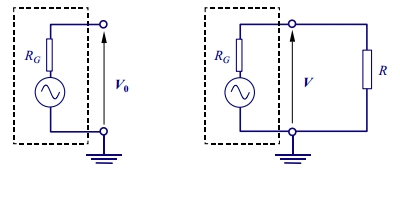
\includegraphics[scale=0.5]{impger.jpg}
    \caption{Circuito representativo para medida da resistência interna do gerador}
  \end{figure}
Primeiro medimos a tensão de saída do gerador de funções conectando-o diretamente ao osciloscópio. Após medir o pico $V_0$, colocamos um resistor em paralelo ao circuito, e obtemos um valor para V. Com essas medidas podemos encontrar um valor para $R_G$, sabendo que temos um divisor de tensão e juntando a Lei de Ohm \footnote{\boxed{V = R\cdot I}}. Logo, \boxed{R_G = R \cdot (\frac{V_0}{V}-1)} e \boxed{\Delta{R_G} = R_G \cdot \sqrt{(\frac{\Delta(\frac{V_0}{V})}{\frac{V_0}{V}-1})^2 + (\frac{\Delta{R}}{R})^2}}, onde \boxed{\Delta{\frac{V_0}{V}} = \frac{V_0}{V} \cdot \sqrt{(\frac{\Delta{V_0}}{V_0})^2 + (\frac{\Delta{V}}{V})^2}}.\\ Portanto, para \boxed{V_0 = 24,8V}\footnote{Escala: 5V}, \boxed{V = 12,2V}\footnote{Escala: 2V} e \boxed{R_{47} = 47,8\Omega , \Delta{R_{47}}=0,6\Omega}\footnote{Dado obtido no experimento I}, temos: \boxed{\Delta{V_0}=0,9940V, \Delta{V}=0,4660V}, resultando em \boxed{\frac{V_0}{V}=2,0328\frac{V}{V}, \Delta{\frac{V_0}{V}}=0,1125\frac{V}{V}} e \boxed{R_G = 49,3672\Omega \pm 5,4154\Omega}.
\item \label{itm:indutor} \textbf{Indutor}: No experimento I, calculamos o valor do indutor utilizado nos experimentos. O resultado foi, \boxed{L = 47,0311mH \pm 4,0174mH}.
\item \label{itm:rindutor} \textbf{Resistência em série do indutor ($R_L$)}: O cálculo de $R_L$ foi apresentado no relatório I, resultando em \boxed{R_L = 46,3\Omega \pm 0,6\Omega}.
\item \label{itm:capacitor} \textbf{Capacitor}: No experimento anterior obtivemos \boxed{C = 0,2236\mu F \pm 0,0191\mu F}.
\item \label{itm:r47} \textbf{Resistor de 47$\Omega$}: \boxed{R_{47} = 47,8\Omega \pm 0,6\Omega}
\end{enumerate}
\subsection{Circuito RC}
\subsubsection{Integrador}
Um circuito integrador é um componente eletrônico contendo elementos, como fonte de tensão[\ref{itm:rger}], resistor[\ref{itm:r47}] e capacitor[\ref{itm:capacitor}].
  \begin{figure}[!htb]
    \centering
    \label{impger}
    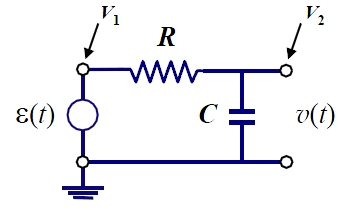
\includegraphics[scale=0.5]{integrador.jpg}
    \caption{Circuito integrador ou Filtro passa-baixa}
  \end{figure}
\begin{enumerate}[I]
\item \textbf{Lei de Kirchoff}: Aplicando a lei de Kirchoff para malhas teremos: \boxed{\varepsilon(t) = R\cdot i(t) + v_c(t)}\footnote{Lembrando que \boxed{I_c(t) = C \cdot \frac{\mathrm d V(t)}{\mathrm d t}}}
\item \textbf{Integrador}: No cálculo acima obtemos: \boxed{v(t)\approx v_0(t) + \frac{1}{RC} \int_{t_0}^{t} \varepsilon(t)dt. }
PAREI AQUI ....FALTA A DEDUCAO DE UM PASSA-BAIXA
\end{enumerate}
\end{document}


